\documentclass{article} % For LaTeX2e
\usepackage{nips13submit_e,times}
\usepackage{hyperref}
\usepackage{url}
\usepackage{graphicx}
\graphicspath{ {images/} }
%\documentstyle[nips13submit_09,times,art10]{article} % For LaTeX 2.09


\title{Machine Learning Milestone}


\author{
Deric Pang \\
\texttt{dericp@cs.washington.edu} \\
\And
Saidutt Nimmagadda \\
\texttt{nimmas@cs.washington.edu} \\
}

% The \author macro works with any number of authors. There are two commands
% used to separate the names and addresses of multiple authors: \And and \AND.
%
% Using \And between authors leaves it to \LaTeX{} to determine where to break
% the lines. Using \AND forces a linebreak at that point. So, if \LaTeX{}
% puts 3 of 4 authors names on the first line, and the last on the second
% line, try using \AND instead of \And before the third author name.

\newcommand{\fix}{\marginpar{FIX}}
\newcommand{\new}{\marginpar{NEW}}

\nipsfinalcopy % Uncomment for camera-ready version

\begin{document}


\maketitle

\begin{abstract}
Our project investigates the task of recognizing handwritten digits. Our initial
project proposal involved reading three papers [1]-[3] and determining which
techniques to use to achieve our task.
\end{abstract}

\section{Project Description}

The data for our project was taken from the MNIST dataset. As written on the
Kaggle competition website, ``The MNIST
('Modified National Institute of Standards and Technology') dataset
is a classic within the Machine Learning community that has been extensively
studied. More detail about the dataset, including Machine Learning algorithms
that have been tried on it and their levels of success, can be found at
http://yann.lecun.com/exdb/mnist/index.html.''

Simply put, we aim to take pixel data from gray-scale images of hand-drawn digits
and classify the digit as a number from 0 to 9.

\section{Progress}

\subsection{Readings}
The readings were helpful in directing us towards the techniques that we should
try to implement. We understood from the
conclusions of the Lecun paper [1] that the k-Nearest Neighbors algorithm would not
only pose serious scaleability difficulties when it came to runtime and memory
usage, but it would also be a comparatively unreliable classifier.

Our findings from the milestone portion of the project confirms this, with our implementation
of k-NN taking a good amount of time (roughly 5 minutes) to run over less than
10 percent of the total dataset. In addition, we only achieved classification
errors of roughly 10 
to 20 percent. When we implement a convolutional neural network, like LeCun did
in his paper, we expect a decrease in runtime and memory usage (which
would promote scaleability), as well as a decrease in classification error.

\subsection{k-NN}
We have implemented a classifier using $k$-nearest neighbors regression. In
order to determine the best value of $k$ to use, we implemented cross-validation
using an 80-20 split.

The first issue we ran into was the massive runtime needed to run k-nn over such
a large model (the training set has 42,000 points). Given runtime constraints,
we ran the algorithm on 10\% of the training set.
For each value of $k$, we found the classification error on the validation set.

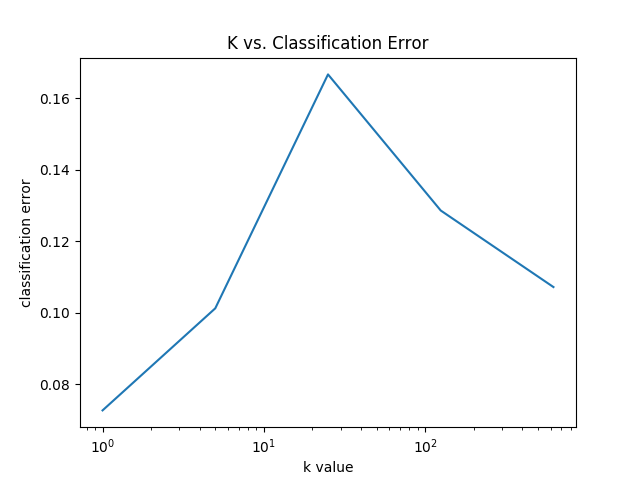
\includegraphics{k-nn.png}



\subsubsection*{References}

\small{
  [1] LeCun, Yann, et al. "Comparison of learning algorithms for handwritten
  digit recognition." International conference on artificial neural networks.
  Vol. 60. 1995.	

  [2] Maji, Subhransu, and Jitendra Malik. "Fast and accurate digit
  classification." EECS Department, University of California,
  Berkeley, Tech. Rep. UCB/EECS-2009-159 (2009).

  [3] Sundaresan, Vishnu, and Jasper Lin. "Recognizing Handwritten Digits and
  Characters." (1998).
}

\end{document}
